
% This defines a new TeX boolean 'isflight' that is true iff we're making the *flight* manual, not the preflight
\newif\ifisflight
% same but for the portapotties events list
\newif\ifisporto

% Type 1 fonts
\usepackage[T1]{fontenc}

% for emojii support

% trying for direct emoji support
\usepackage{fontspec}
\usepackage{fontawesome}
\usepackage{fontawesome5}

\newfontfamily\DejaSans{DejaVu Sans}

% Include figures
\usepackage{graphicx}

% For SI Units; mostly to use for degrees.
\usepackage{siunitx}

%multirow support for tables
\usepackage{multirow}

% For nice slanted fractions
\usepackage{xfrac}


% for TODO items
\usepackage[usenames,dvipsnames]{xcolor}
% \usepackage[disable]{todonotes}
\usepackage[]{todonotes}
%% green bubbles for BOD todos
\newcommand{\bod}[2][]{\todo[color=green,#1]{#2}}

% Fancy tables
\usepackage{booktabs}

% Allow for use of multiple columns
\usepackage{multicol}

% This provides a wee bit better typography
\usepackage{microtype}

% Some basic math 
\usepackage{calc}

% Make the labels for labeling lists look nicer with a sans serif font
\addtokomafont{labelinglabel}{\sffamily}

% This to grab the \square used in checklists
\usepackage{amssymb}

% Better lists
\usepackage{enumitem}

% Make a checklist environment
\newlist{checklist}{itemize}{2}
\setlist[checklist]{label=$\square$}

% \usepackage{libertine}
\renewcommand{\familydefault}{\sfdefault}

% For better appendix support
% TODO Not sure if we want appendices; overkill?
\usepackage{appendix}

% sideways figures
\usepackage{rotating}

% figures wrapped in text
\usepackage{wrapfig}

% % caption next to figure (SCfigure)
% \usepackage{sidecap}

% % another attempt to get caption next to image
% \usepackage{paracol}

% Glossary definitions and acronyms common to pre-flight manual and survival guide
%
% A list of glossary terms and acronyms
%
% Shared between pre-flight manual and survival guide
%

%%
%% Begin glossary stuff
%%
% \usepackage[acronym,style=long3colborder]{glossaries}
\usepackage[acronym]{glossaries}

\usepackage{glossary-longbooktabs}

% First use use full name of acronym, then the abbreviated.
\setacronymstyle{long-short}

% From https://en.wikibooks.org/wiki/LaTeX/Glossary#Defining_glossary_entries
% To support things that are both acronyms and glossary items, e.g., "MOOP."
\usepackage{xparse}
\DeclareDocumentCommand{\newdualentry}{ O{} O{} m m m m } {
  \newglossaryentry{gls-#3}{name={#5},text={#5\glsadd{#3}},
    description={#6},#1
  }
  \makeglossaries
  \newacronym[see={[Glossary:]{gls-#3}},#2]{#3}{#4}{#5\glsadd{gls-#3}}
}

% \makenoidxglossaries
\makeglossaries

% \newglossaryentry{moopgl}{
% name = {Matter Out of Place},
% description = {Anything not part of the natural environment, such as glitter, litter, bottle caps, and cigarette butts.}
% }

\newdualentry{moop} % label
  {MOOP}            % abbreviation
  {Matter Out of Place}  % long form
  {Trash, litter, things lost or left behind, things on the ground that should not be there.} % description
  

\newglossaryentry{rangers} {
name = {Rangers},
description = {A volunteer empowered to address safety concerns, mediate disputes, and resolve conflicts when they cannot be resolved by the persons involved}
% This is already in the team description for rangers
% \begin{labeling}{khaki}
% \item[alpha:] novice ranger
% \item[dirt:] (as in older than ...) an experienced ranger
% \item[khaki:] a Ranger that stays at HQ as a point-of-contact
% \end{labeling}}
}

\newglossaryentry{effigy} {
name = {effigy},
description = {The main art piece to be burned Saturday night.}
}

\newglossaryentry{graywater} {
name = {gray water},
description = {Water left-over from cleaning dishes or bathing.}
}

\newglossaryentry{crew} {
name = {crew},
description = {You.}
}

\newglossaryentry{gifting} {
name = {gifting},
description = {Giving food, an item, or a service without any expectation of reciprocity}
}

\newglossaryentry{mudburn} {
name = {Mud Burn},
description = {A burn characterized by extreme mud due to inclement weather}
}

\newglossaryentry{artcar} {
name = {Art Car},
description = {See: \gls{mutantvehicles}}
}

\newglossaryentry{mutantvehicles} {
name = {Mutant Vehicles},
description = {A motorized conveyance that is radically, stunningly, and safely modified. See also: \gls{artcar}}
}

\newglossaryentry{centercamp} {
name = {Center Camp},
description = {Host to many different musical experiences, performance art, and educational classes.}
}

\newglossaryentry{conclave} {
name = {Conclave},
description = {The Saturday night fire performance delivered by any interested and competent participants.}
}

\newglossaryentry{cockpit} {
name = {COCKpit},
description = {The main information station to visit when you have questions and need answers. There is also a huge map so you can find yourself. It's the home base for Volunteer Coordination, First Aid, \gls{lamplighters}, and \gls{lnt}}
}

\newglossaryentry{groundcontrol} {
name = {Ground Control},
description = {Department of Public Works Headquarters.}
}

\newglossaryentry{missioncontrol} {
name = {Mission Control},
description = {Rangers Headquarters.}
}

\newglossaryentry{shiftlead} {
name = {shift lead},
description = {some teams operator on a 24 $\times$ 7 schedule that is divided into shifts; a shift lead is one designated to be in charge of a given team for a shift}
}


\newglossaryentry{darkwad} {
name = {darkwad},
description = {Someone who is running around at night with no light or glow on. It gets dark out there. Real dark.}
}

\newglossaryentry{darksideofthemoon} {
name = {Dark Side of the Moon},
description = {Open camping located on the extreme eastern edge of the site well within the tree line.  Ideal for introverts without a theme camp, or those averse to the sun.}
}

\newglossaryentry{defaultworld} {
name = {default world},
description = {The rest of the world that is not a burn.}
}

% dual entry
\newdualentry{dmv} 
{DMV}
{Department of Mutant Vehicles}
{The volunteers who review and register \gls{mutantvehicles}, giving them permission to drive during the event.}


%dualentry
\newdualentry{dpw} 
{DPW}
{Department of Public Works}
{The team responsible for overseeing construction of the infrastructure, managing inventory, completing construction projects, overseeing Build Weekend and Tear Down, fueling the Effigy and Temple, and generally working behind the scenes during the event to deal with infrastructure issues as they arise. Also called Public Works.}

\newglossaryentry{education} {
name = {education},
description = {See: \glspl{greeter}}
}

\newglossaryentry{effigyburnfield} {
name = {Effigy Burn Field},
description = {This is where the effigy gets burnt.}
}

\newglossaryentry{templefield} {
name = {Temple Field},
description = {This is where the temple gets burnt.}
}

\newglossaryentry{eventleads} {
name = {event leads},
description = {This the team of volunteers who manage the event, and whom facilitate community needs. They are selected by the Board of Directors, which in turn is elected by the \gls{ttm} community.}
}

\newglossaryentry{gate} {
name = {Gate},
description = {The entrance to the burn where your ticket and ID will be checked, and where you will sign a waiver.}
}

\newglossaryentry{greeter} {
name = {Greeter},
description = {A friendly volunteer that will welcome you to the Burn, give you your \gls{swag}, and provide \gls{education} about the 10 (11) Principles. }
}

\newglossaryentry{groundscore} {
name = {ground score},
description = {\gls{moop} that is useful to you --- if you find something that someone dropped and you keep it, it's a ground score. If it looks valuable don’t be a dick, take it to lost and found. }
}

\newglossaryentry{lamplighters} {
name = {lamp lighters},
description = {The volunteer group that lights lanterns each night to illuminate some of the roads.}
}

\newglossaryentry{launchpad} {
name = {launchpad},
description = {Area where \gls{gate}/\glspl{greeter} are located.}
}

\newglossaryentry{temple} {
name = {temple},
description = {this is the art structure burned on the last night (though Euphoria has kindly donated their temple, which is to be burned Friday night)}
}

% dual entry
\newdualentry{lnt} 
{LNT}
{Leave No Trace}
{The concept that we should leave the property in better shape than we found it. It can also be verbed, as in ``Hey, I'm going to LNT the campsite after everyone packs up.'' }

\newglossaryentry{moonrangerstation} {
name = {Moon Ranger Station},
description = {Meeting point for Ranger Training.}
}

\newglossaryentry{opencamping} {
name = {open camping},
description = {where camping is permitted by participants who do not have a pre-assigned Theme Camp.}
}

\newglossaryentry{perimeter} {
name = {perimeter},
description = {Predetermined areas around the structure combustion events (Effigy, Temple, etc) that are staffed by volunteers to keep observers at a safe distance.}
}

% dual entry
\newdualentry{poop}
{POOP}
{Person Out of Place}
{People who are not where they should be. If you see someone passed out on the ground in the middle of the field, they may be drunk or having a medical emergency. Check and see if they are OK. If they want to be there, it's at their own risk if they get run over by a golf cart; but we try to get these people back to their camps.}

\newglossaryentry{sparklepony} {
name = {sparkle pony},
description = {A derogatory term for burners who show up to the event with little or no food or water, suitcases full of costumes and makeup, who do no work and no volunteering and only exist to look pretty, have fun, and party. They are often fashionably attired since they packed nothing but costumes.}
}

\newglossaryentry{swag} {
name = {swag},
description = {A memento from a burn, often wearable. You get swag for attending from \glspl{greeter}, often swag from your volunteer teams, and people you meet may gift you swag they made for the burn.}
}

\newglossaryentry{teamleads} {
name = {team leads},
description = {The people who head up each team that makes the burn happen.}
}

\newglossaryentry{tenprinciples} {
name = {Ten Principles},
description = {The ten core guiding concepts of most burns. }
}

\newglossaryentry{themecamp} {
name = {theme camp},
description = {A group of people camping together in a pre-assigned spot who often have common bonds and shared activities.}
}

\newglossaryentry{tbass} {
name = {Tranquility Base},
description = {(A.k.a., Tbase/Sanctuary) A dedicated space for those who may need an environment or area in which to better acclimate or adjust to the Burn.}
}

\newglossaryentry{village} {
name = {village},
description = {A group of Theme Camps sharing a common space and ethos.}
}

\newglossaryentry{eleventhprinciple} {
name = {11th Principle},
description = {The 11th Principle}
}


\newglossaryentry{preflightmanual} {
name = {pre-flight manual},
description = {The document that contains information essential for planning and preparing for \gls{ttm}}
}


\newglossaryentry{survivalguide} {
name = {survival guide},
description = {The document that contains information essential for planning and preparing for \gls{ttm}, and which provides information about events, theme camps, and art during the event.  Essentially, it is the \gls{preflightmanual} plus art, camp, and event listings.}
}


\newglossaryentry{parking} {
name = {Parking},
description = {There is a large parking area at the entrance.}
}

%% Glossary item template
% \newglossaryentry{} {
% name = {},
% sort = {},
% description = {}
% }

%% Glossary dual entry template -- i.e., things that are acronyms *and* glossary entries, like MOOP
% \newdualentry{OWD} % label
%   {OWD}            % abbreviation
%   {One-Way Delay}  % long form
%   {The time a packet uses through a network from one host to another} % description

\setglossarysection{subsection}


% acronym tag, short name, long name
\newacronym{ttm}   {TTM}      {To the Moon}
\newacronym{bod}   {BOD}      {Board of Directors}
\newacronym{leo}   {LEO}      {Law Enforcement Officer}
\newacronym{vc}    {VC}       {Volunteer Coordination}
\newacronym{gtfio} {GTFIO}    {Get the Fuck In and Out}
\newacronym{love}  {L.O.V.E.} {Lunar Orbit Vehicle Extraction}
\newacronym{pipo}  {PIPO}     {Pack in/pack out}
\newacronym{el}    {EL}       {Event Lead}
% \newacronym{SHORTNAME}  {ABBREV}  {LONGNAME}



%%
%% End glossary stuff
%%



% set text in a shape
\usepackage{shapepar}

% add H placement option for floats which really puts them where you want them
% \usepackage{float}
\usepackage{floatrow}

% absolute position for text (titlepage)
\usepackage[absolute]{textpos}
 \setlength{\TPHorizModule}{1mm}%
 \setlength{\TPVertModule}{1mm}%

% sideways figure/"H" placement 
\usepackage{float}

% This is for fancy schmancy ornaments
\usepackage{pgfornament}
\usepackage{tikz}
\usetikzlibrary{calc,matrix,shapes}

%%
%% For setting the title page background
%%
\usepackage{eso-pic}

%% fancy table alignment, used to create formatting for headers in events and camps with icons
\usepackage{tabularray}
\SetTblrInner{colsep=0pt}

% \usepackage{tasks}

\definecolor{red2022}{HTML}{C0062C}

\newcommand\LetterSizeTitlePic{%
\put(0,0){%
\parbox[b][\paperheight]{\paperwidth}{%
\vfill
\centering
{\includegraphics[width=\paperwidth,height=\paperheight]{images/cover-art/2022coverpageletter}}%
\vfill
}}}

\newcommand\HalfLetterSizeTitlePic{%
\put(0,0){%
\parbox[b][\paperheight]{\paperwidth}{%
\vfill
\centering
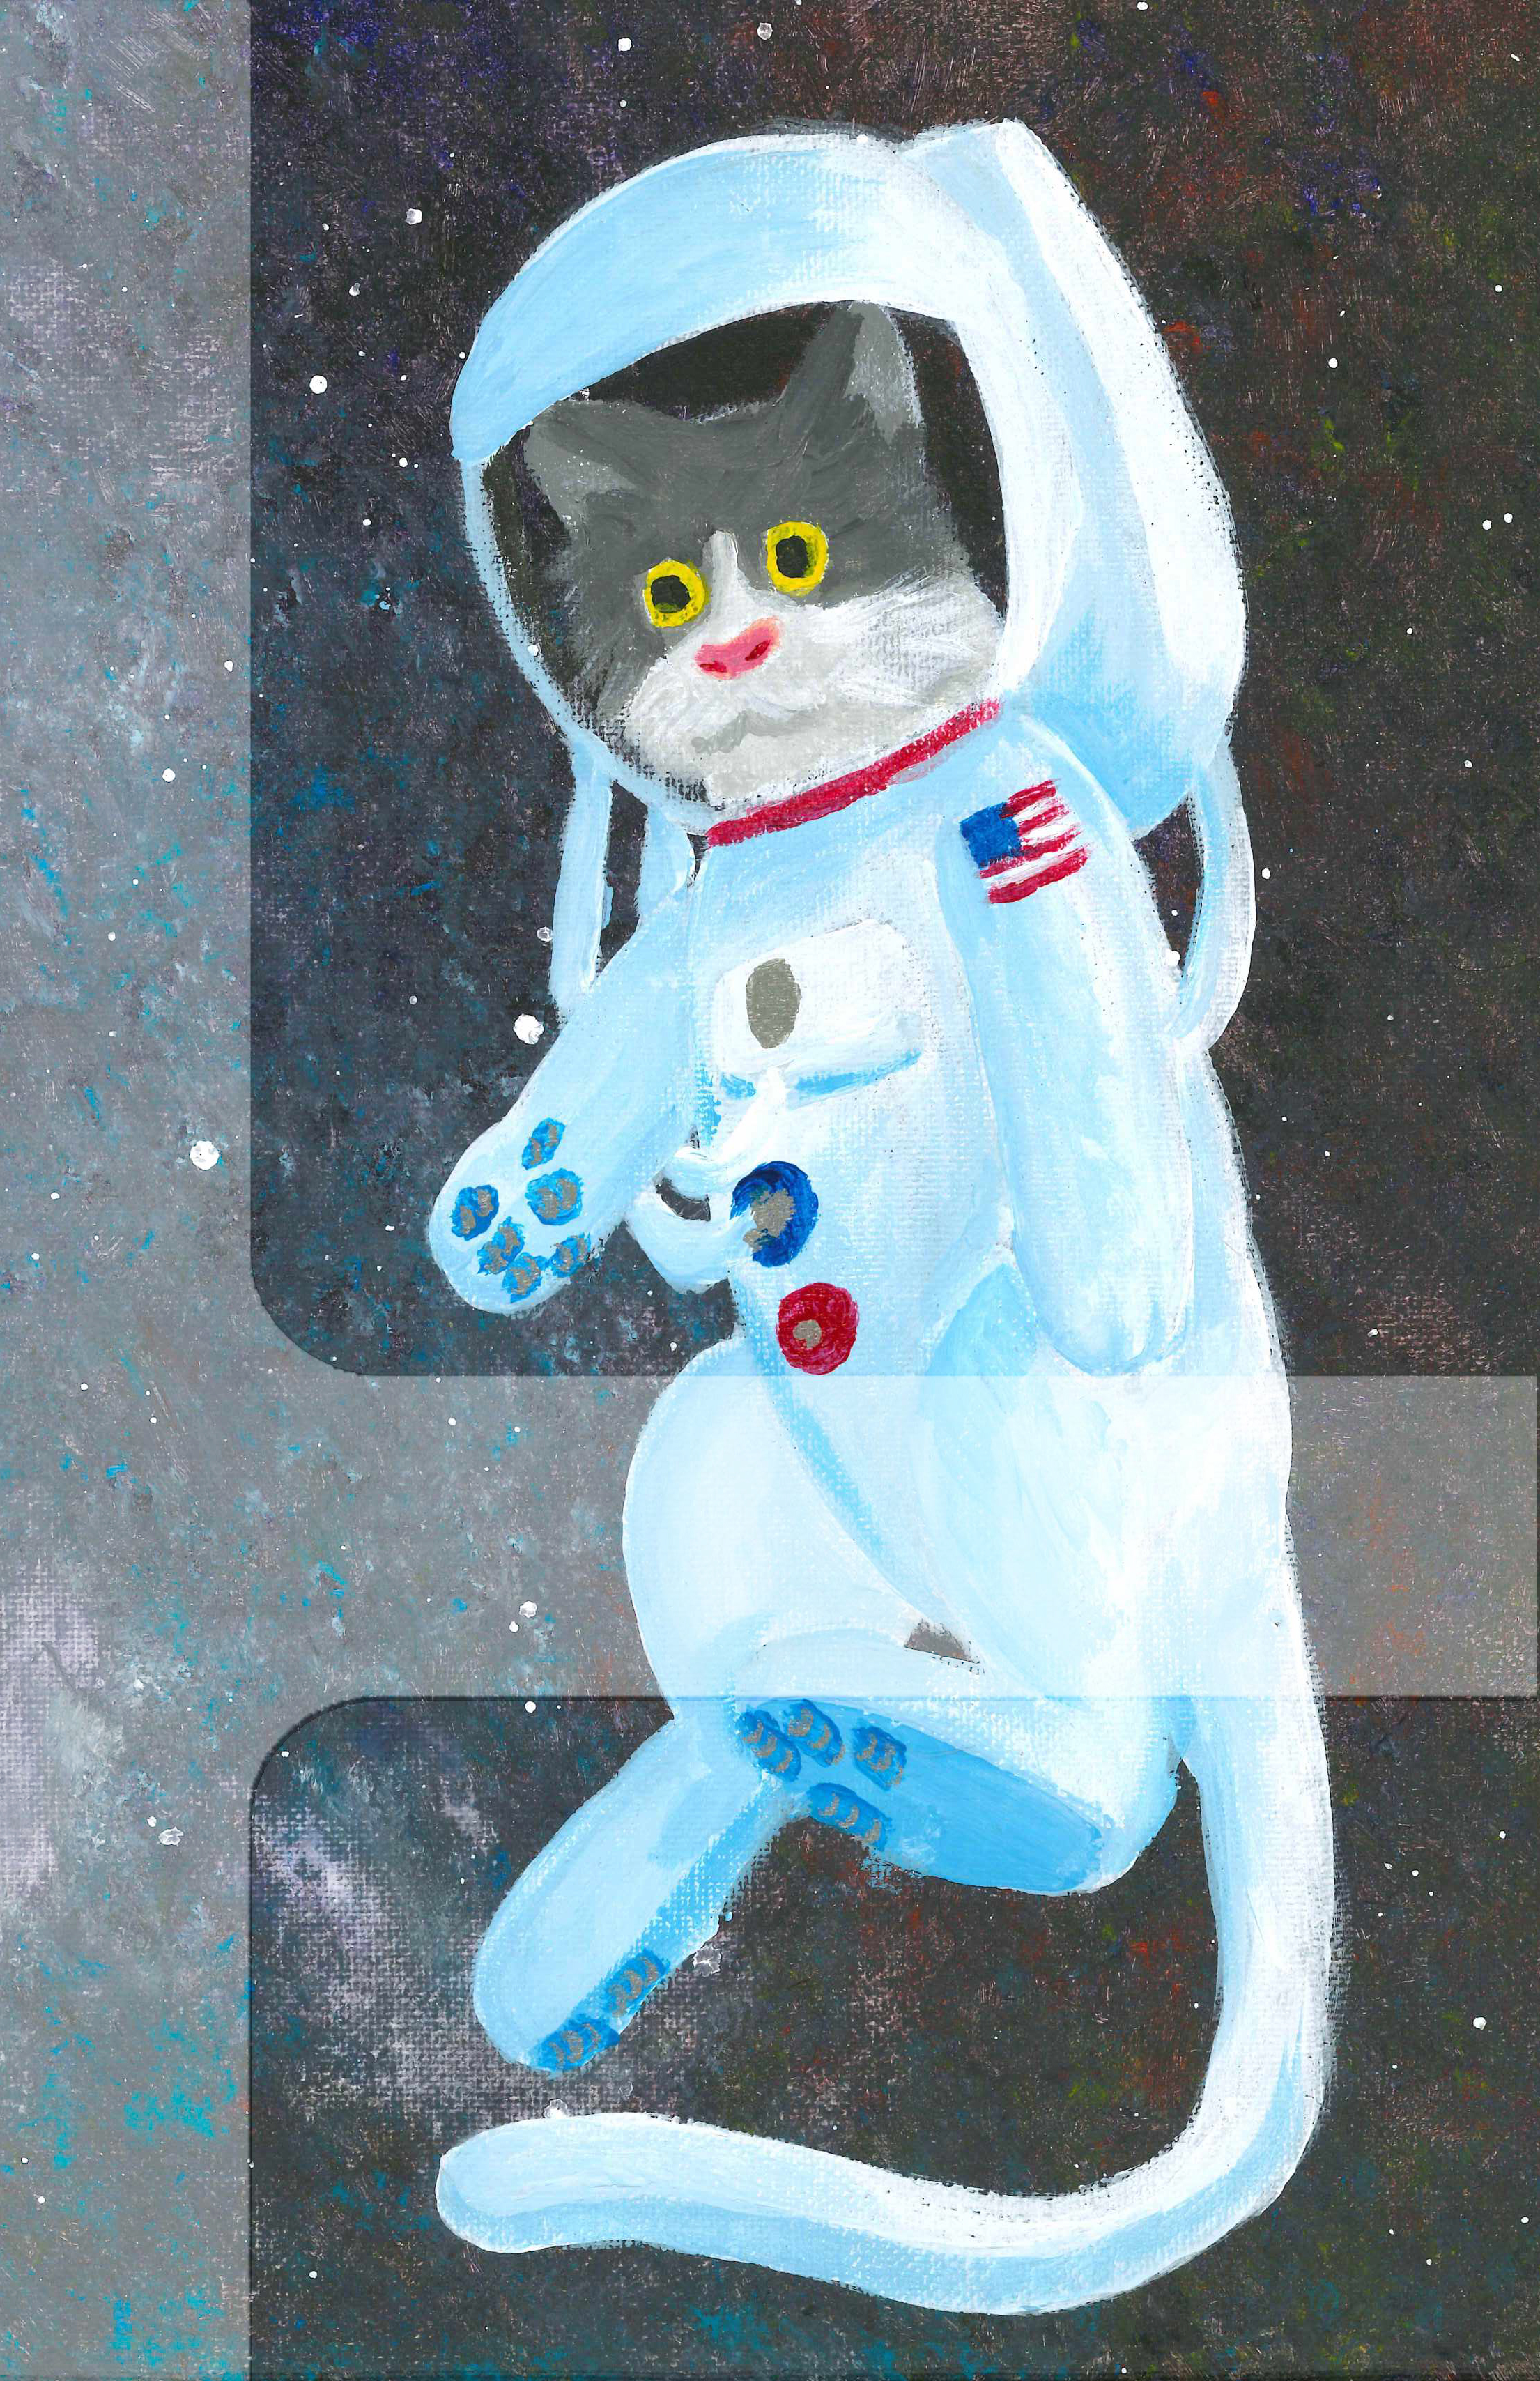
\includegraphics[width=\paperwidth,height=\paperheight]{images/cover-art/2022coverpageHalfLetter}%
\vfill
}}}

% NASA image from https://svs.gsfc.nasa.gov/vis/a000000/a003600/a003686/SPflyover_v07_still.5000.jpg
\newcommand\ThemePic{%
\put(0,0){%
\parbox[b][\paperheight]{\paperwidth}{%
\vfill
\centering
% \includegraphics[width=\paperwidth,height=\paperheight]{images/moon_bg.jpg}%
\includegraphics[width=\paperwidth,height=\paperheight]{images/cover-art/landercroppedmore.jpg}%
\vfill
}}}

%% Consistent notation for am and pm, easy to change right here :D
\usepackage{xspace}
\newcommand{\am}{am\xspace}
\renewcommand{\pm}{pm\xspace}

% Support for URLs and document links
\usepackage[]{hyperref}
% \hypersetup{colorlinks=true,allcolors=[rgb]{0,.5,.7}}
\hypersetup{
  colorlinks   = true, %Colours links instead of ugly boxes
  urlcolor     = [rgb]{0,.5,.7}, %Colour for external hyperlinks
  linkcolor    = [rgb]{0,.5,.7}, %Colour of internal links
  citecolor   = [rgb]{0,.5,.7} %Colour of citations
}
% \hypersetup{colorlinks=false}


%% Remove leading space in new paragraphs
\setlength{\parindent}{0pt}
\setlength{\parskip}{.7em}
\widowpenalty 10000
\clubpenalty 10000



\frenchspacing % eliminate extra spaces after periods

% \newcommand{\ttmfont}[1]{\fontsize{2.3cm}{1cm}\selectfont{\textbf{\textcolor{red2022}{\sffamily#1}}}}
% \newcommand{\guidetypefont}[1]{\fontsize{1.2cm}{1.4cm}\selectfont{\textbf{\textcolor{red2022}{\sffamily#1}}}}
% \newcommand{\guideversionfont}[1]{\fontsize{.95cm}{1.3cm}\selectfont{\textcolor{red2022}{\sffamily#1}}}
% \newcommand{\locationfont}[1]{\fontsize{0.6cm}{.5cm}\selectfont{\textbf{\textcolor{red2022}{\sffamily\uppercase{#1}}}}}
